\section{Badania}
W~niniejszym rozdziale opisany został przebieg przeprowadzonych badań oraz analiza ich wyników. W~kolejnych podrozdziałach zostaną przedstawione kolejne różne eksperymenty. Dokładne otrzymane wyniki znajdują się na~dołączonej do pracy płycie~CD w~odpowiednich plikach, o~nazwach zgodnych z~podrozdziałem opisującym dane badanie i~jego wyniki.

%\subsection{Opóźnienia pojedynczego odcinka sieci}
%\subsection{Wpływ topologi na opóźnienia}
\subsection{Czas stabilizacji sieci po odłączeniu i~podłączeniu dowolnego urządzenia}
Badanie miało na~celu sprawdzenie czy zgodnie z~zapewnieniami producenta faktycznie możliwe jest rozłączanie i~podłączanie urządzeń do~sieci ,,w locie'' bez większych problemów i~bez konieczności żadnej dodatkowej ingerencji. Do przeprowadzenia pomiarów autor odłączał wtyczkę i~podłączał ja~ponownie do~gniazda. Oczywiście metoda da~może mieć minimalny wpływ na~dokładność dokonywanych pomiarów, ale zdaniem autora jest on minimalna ze względu na to, że od~momentu odłączenia do wykrycia tego faktu przez urządzenie nadzorujące pracę sieci mija pewien czas, który w optymistycznym przypadku może być krótszy niż sam proces ingerencji autora. Aby poprawić dokładność można by zastosować specjalnie stworzone samodzielnie urządzenie co zostanie opisane w~perspektywach rozwoju niniejszej pracy. Wszystkie zmierzone czasy oraz treści komunikatów zostały odczytane w~środowisku TwinCAT System Manager, przykładowy został przedstawiony na Rysunku~\ref{}.

\subsubsection{Pojedyncze urządzenie}
Eksperyment miał na~celu sprawdzenie jak szybko po~odłączeniu i~ponownym podłączeniu pojedynczego węzła sieci zaczyna on~funkcjonować poprawnie. Zaburzoną pracę sieci przedstawiono na~Rysunku~\ref{one_slave}, który został wygenerowany przy użyciu środowiska TwinCAT System Manager i jest to~jedna z~jego opcji. Jak widać wybrany został węzeł końcowy w topologii.

\begin{figure}[!htb] 	\centering 	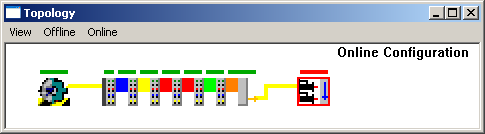
\includegraphics[width=0.9\textwidth]{images/topologyCXerror} \caption{Topologia stanowiska z odłączonym jednym węzłem} \label{one_slave} \end{figure}
%2,6s do 2,7s

Wartości zmierzone po ówczesnej obróbce zostały zebrane i przedstawione w Tabeli~\ref{badania:wyniki:stabilizacja_jeden}.
\begin{table}[!htb]
\begin{center}
\begin{tabular}{| c | c | c | c |}\hline
\textbf{Liczba próbek} & \textbf{Wartość średnia} & \textbf{Wartość minimalna} & \textbf{Wartość maksymalna} \\\hline\hline
20 & 2.678s & 2.654s & 2.774s \\\hline
\end{tabular}
\end{center}
\vspace*{-6mm}
  \caption{Wyniki przeprowadzonego badania}
	\label{badania:wyniki:stabilizacja_jeden}
\end{table}
Na podstawie zmierzonych wartości oraz po dokonaniu stosownych obliczeń udało się wygenerować wykres przedstawiony na Rysunku~\ref{badania:wykres:stabilizacja_jeden}
\begin{figure}[htbp]
 \centering
 \begin{tikzpicture}[x=0.5cm,y=2cm]
  \tikzstyle{background grid}=[draw, black!50,step=.25cm]
	\draw[-latex, thin, draw=gray] (0,0)--(20,0) node [right] {$x$};
	\draw[-latex, thin, draw=gray] (0,0)--(0,4) node [above] {$t[s]$};
	%\draw [dotted, gray, step=0.5cm] (0,0) grid (20,4);
 
	\draw[thick] (0,2.678)--(20,2.678) node[left=10cm] {2,678};
	\draw[thin, dotted] (0,2.664)--(20,2.664) node[below] {min};
	\draw[thin, dotted] (0,2.774)--(20,2.774) node[above] {max};
		
	\node at (1, 2.664) {\textbullet};
	\node at (2, 2.664) {\textbullet};
	\node at (3, 2.654) {\textbullet};
	\node at (4, 2.664) {\textbullet};
	\node at (5, 2.654) {\textbullet};
	\node at (6, 2.774) {\textbullet};
	\node at (7, 2.764) {\textbullet};
	\node at (8, 2.664) {\textbullet};		
	\node at (9, 2.654) {\textbullet};
	\node at (10, 2.664) {\textbullet};
	\node at (11, 2.654) {\textbullet};
	\node at (12, 2.664) {\textbullet};
%	\node at (13, 2.774) {\textbullet};
%	\node at (14, 2.774) {\textbullet};
%	\node at (15, 2.774) {\textbullet};
%	\node at (16, 2.774) {\textbullet};							
%	\node at (17, 2.774) {\textbullet};
%	\node at (18, 2.774) {\textbullet};
%	\node at (19, 2.774) {\textbullet};
%	\node at (20, 2.774) {\textbullet};
					
\end{tikzpicture}
\caption{Pomiary czasu ponownego podłączenia oraz obliczona wartość średnia}
\label{badania:wykres:stabilizacja_jeden}
\end{figure}

Jak wykazują wyniki przeprowadzonego eksperymentu faktycznie można pozwolić sobie na odłączenie i~ponowne podłączenie pojedynczego węzła sieci ,,w locie''. Czas potrzebny na stabilizację połączenia po jego utracie jest zdaniem autora zadowalający. Analiza uzyskanego wykresu pozwala zauważyć, że różnice pomiędzy kolejnymi iteracjami eksperymentu są stosunkowo małe i~wpływ na~nie może mieć w~większości zastosowana metoda pomiarowa. Jak widać większość wyników skupia się w~otoczeniu wartości średniej.

\subsubsection{Wyspa z modułami I/O}
Eksperyment miał na~celu sprawdzenie jak szybko po~odłączeniu i~ponownym podłączeniu wyspy z~dołączonymi kilkoma modułami wejścia/wyjścia zaczynają funkcjonować poprawnie wszystkie węzły. Zaburzoną pracę sieci przedstawiono na~Rysunku~\ref{coupler}.
\begin{figure}[!htb] 	\centering 	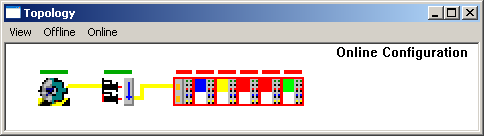
\includegraphics[width=0.9\textwidth]{images/topologyCPerror} \caption{Topologia stanowiska z odłączoną wyspą} \label{coupler} \end{figure}
%1,5s wyspa i każdy kolejny moduł I/O z opóźnieniem 4ms

Wartości zmierzone po ówczesnej obróbce zostały zebrane i przedstawione w Tabeli~\ref{badania:wyniki:stabilizacja_wyspa}.
\begin{table}[!htb]
\begin{center}
\begin{tabular}{| c | c | c | c |}\hline
\textbf{Liczba próbek} & \textbf{Wartość średnia} & \textbf{Wartość minimalna} & \textbf{Wartość maksymalna} \\\hline\hline
7 & 1.51+5*0.02 & 1.45+5*0.024 & 1.56+5*0.02 \\\hline
\end{tabular}
\end{center}
\vspace*{-6mm}
  \caption{Wyniki przeprowadzonego badania}
	\label{badania:wyniki:stabilizacja_wyspa}
\end{table}
Na podstawie zmierzonych wartości oraz po dokonaniu stosownych obliczeń udało się wygenerować wykres przedstawiony na Rysunku~\ref{badania:wykres:stabilizacja_wyspa}. Różnymi kolorami są oznaczone kolejne iteracje badania, a kolejne punkty tego samego koloru przedstawiają kolejne węzły.
\begin{figure}[htbp]
 \centering
 \begin{tikzpicture}[x=0.5cm,y=10cm]


 \draw[latex-latex, thin, draw=gray] (0,1.25)--(20,1.25) node [right] {$x$}; % l'axe des abscisses
 \draw[latex-latex, thin, draw=gray] (0,1.25)--(0,2) node [above] {$y$}; % l'axe des ordonnées
 \draw[thick] (0,1.5)--(20,1.58); % l'axe des abscisses

    \foreach \i in {0,...,20}{% 
\foreach \Point in {(\i ,1.5+0.004*\i)}{
    \node at \Point {\textbullet}; } ;}     

% to ensure that the points are being properly centered:
\draw [dotted, gray] (0,1.25) grid (20,2);

\end{tikzpicture}
\caption{Współczynnik wykorzystania kanału transmisyjnego w Ethernecie (dwa pierwsze wykresy od lewej strony) i EtherCAT}
\label{etherCAT:wykorzystanie}
\end{figure}

Jak widać zwiększenie liczby odłączanych i~podłączanych ponownie węzłów nie~wpłynęło w sposób negatywny na~możliwość dokonywania tej operacji w czasie pracy sieci. Ciekawy wydaje się równy czas wynoszący 2ms pomiędzy podłączeniem się pierwszego urządzenia z~zestawu, a~każdym kolejnym. Tak więc liczba modułów wejścia/wyjścia ma~proporcjonalnie mały wpływ na czas potrzebny do ustabilizowania się całego zdalnego zestawu.

\subsubsection{Problemy}
W~czasie dziesiątek przeprowadzonych w~tym badaniu testów ku~zaskoczeniu autora wystąpiły sytuację w~których sieć nie~powróciła już samoczynnie do~prawidłowego działania. Jest to sprzeczne z zapewnieniami twórców standardu i~dlatego wszystkie te~przypadki zostaną tu zawarte i~opisane.

\begin{enumerate}
\item Device 2 (EtherCAT (v2.10 only)': 'INIT to PREOP' failed! Error: 'read slave count'. Communication Error '0x707 (1799)'. \\[1mm]
ADS, problem ze stanem urządzenia
Okazało się, ze problem ten można rozwiązać w~miarę prosto bez potrzeby restartowania całego stanowiska poprzez wymuszenie zmiany stanu węzła nadrzędnego z~INIT na OP.
\end{enumerate}

\subsection{Badania niewykonalne}

\subsubsection{Zbadanie innych topologii}

\subsubsection{Zbadanie opóźnień na poziomie transmisji pojedynczych ramek}
%Różne kable
%Długość kabla
%
%Połączyć do jednego sterownika oba napędy kolejno i zrobić coś na zasadzie inkrementacji i sprawdzić czy się przypadkiem nie rozjedzie
%
%Mamy opóźnienie na jednym odcinku
%
%Ewentualnie jeden kabel można zamienić na dłuższy i sprawdzić czy nie ma różnicy.
%
%Wymyślić jak sprawdzić czas ponownego włączenia do sieci.